% !TeX spellcheck = de_DE
\chapter{Systemdesign}
\label{sec:design}
Dieser Kapitel erklärt die Anforderungen an der Software, die unten detailliert erklärt werden. Nachdem die Aufgabestellung des Projekts wurde von PSE-Labor veröffentlicht und mit Autorin der Abschlussarbeit besprochen und alle Unklarheiten geklärt und auf die Lieferung der Hardware in das PSE-Labor gewartet wurde, wurde der erste notwendige Schritt angefangen: Systemdesign. Im Rahmen des Systemdesigns werden die Struktur und Zusammenhänge der Elemente des zu entwickelnden Systems untersucht. Das Ergebnis dieser Untersuchung enthält genügend Informationen, um das System zu implementieren. 


\section{User Stories}
\label{sec:design:user_stories}
Zuerst wurden die User Stories erstellt, die eine diskutierte Darstellung der Absicht (Endbenutzer muss/will so etwas tun) zeigen können. Es ist mithilfe der User Stories zu klären, was die zu entwickelnde Datenbank leisten soll. Es wird auf die Frage konzentriert, welche Daten in der Datenbank gespeichert werden sollen. 
Der Text der User Story selbst sollte die Rolle / Aktionen des Benutzers im System, seine Bedürfnisse und den Gewinn erläutern, den der Benutzer nach dem Auftreten der Story erhält. Zum Beispiel: Wie \textit{<Benutzerrolle / Charakter>, ich <möchte etwas bekommen>, <für diesen und jenen Zweck>}. Während des Schreibens der User Story wurden zwei Gruppe von Stakeholders definiert: die Studierende (Beuth Studentinnen und Studenten) und der Admin (PSE-Labor Mitarbeitern). Es wurden die folgenden User Stories erstellt (für die Verwaltung des Projekts  der Abbildung \ref*{fig:stories} zu sehen), die später während der Entwicklungsphase implementiert wurden:
\begin{itemize}
	\itemsep-1.2em 
	\item As a student, I want \textbf{to loan a board} so I can work at lab
	\item As a student, I want \textbf{to loan a board} so I can work at home
	\item As a student, I want \textbf{to list boards assigned to me} so that I am sure I to return
	\item As a student, I want \textbf{to return a board from lab work} so that I can loan again
	\item As a student, I want \textbf{to return a board from home work} so that I can loan again
	\item As a student, I want \textbf{to initiate session} so I can loan a board
	\item As a lab admin, I want \textbf{to mark a board} so it can be loaned for home or for lab
	\item As a lab admin, I want \textbf{to terminal session} with timeout so that students can use the loan station
	\item As a lab admin, I want \textbf{to block a student} so that they won't be able to loan a board
	\item As a lab admin, I want \textbf{to see all students} registered on the course so that I can manage their profiles
	\item As a lab admin, I want \textbf{to see all loaned boards} so that I can know their expected return date
	\item As a lab admin, I want \textbf{to register students} so that they are able to loan boards
	\item As a lab admin, I want \textbf{to register new boards} so that thay can be loaned
	\item As a lab admin, I want \textbf{to delete student's record} when semester ends so that they are not stored anymore in database
\end{itemize}


\section{Anforderungen}
\label{sec:design:req}
Die Softwareentwicklung beginnt mit einer Beschreibung der Bedürfnisse und ihrer Analyse. Je genauer und korrekter die Beschreibung der Softwareanforderungen und deren Analyse ist, desto einfacher ist es, alle nachfolgenden Schritte abzuschließen. Das Hauptproblem in dieser Phase ist der Unterschied in den Ansichten des Kunden (in dem Fall der vorliegenden Abschlussarbeit sind die Kunden die PSE-Labor Mitarbeiter) und des Entwicklers (die Autorin der Abschlussarbeit). Es wurde auch die Entscheidung getroffen, mit welchen Hardware ist die Aufgabestellung zu implementieren. Jedoch während der Entwicklung der Register-Client (der einer von drei Bestandsteilen der Software, an dem ein RFID-Leser angeschlossen werden muss), wurde schließlich den RFID-Leser gewechselt. Der Fall ist im Kapitel \ref{sec:register_client:install_rfid} nachzulesen.


Während die meisten neuen Funktionen mithilfe der User Stories aus Anwendersicht definiert werden sollten, ist dies nicht immer machbar oder sogar hilfreich, wenn es zu Sicherheitsfunktionen oder Infrastrukturanforderungen kommt, die nicht kundenorientiert sind. Die Anforderungen sind in der Regel mehr detailliert und das Schreiben dauert länger. Diese gehen oft technisch auf die Funktionsweise der Software ein. Diese Details leiten das Entwicklungsteam dann beim Erstellen eines neuen Features oder einer neuen Funktionalität. Es gibt zwei Arten von Anforderungen: eine funktionale Anforderung, die beschreibt, was ein Softwaresystem tun sollte, und eine nicht funktionale Anforderungen, die Vorgehensweise des Systems einschränken sollte. Während der Analysephase wurden die beiden Arten von Anforderungen definiert. Die manche von diese Anforderungen sind in der unten geschriebenen Liste zu sehen.

\textbf{Funktionale Anforderungen}
\begin{itemize}
	\itemsep-1.2em 
	\item The background color for all windows in the application will be white and have a hexadecimal RGB color value of 0x0000FF.
	\item The colors of design guidelines of Beuth Hochschule will be used
	\item The software automatically validates whether a student is able to loan a board for a homework
	\item The software automatically shows the information about boards they already loaned
	\item Student will see their name after they scanned their valid student card
	\item Student will see board's number after they scanned a Raspberry Board
\end{itemize}

\textbf{Nicht funktionale Anforderungen}
\begin{itemize}
	\itemsep-1.2em 
	\item Users must use for the initial login their student card. Moreover, every next login will be done with the same card. 
	\item Students never allowed to loan home board longer than 1 week (7 calendar days). Such attempt should be reported to the security administrator.
	\item Students never allowed to loan lab board longer than 120 minutes. An the end of the exercise admnistrator should be notified it the board was not returned.
	\item Loan process can not be started if a student was not properly registered on the course
	\item Every unsuccessful attempt by a user to loan/return an item shall be recorded on an audit trail.
	\item Only one active session is allowed for loan/return process. No multi-user mode is intended
	\item If the currect session is inactive longer longer than 60s the session will be terminated and should be restarted
\end{itemize}

Wie es zu sehen ist, sind User Stories ein großartiges und notwendiges Werkzeug. Die User Story selbst ist die Verbindung zwischen der menschlichen Wahrnehmung und der technischen Umsetzung. Mithilfe der Anforderungen können die Betriebsfunktionen und Einschränkungen des Systems beschrieben werden, die seine Funktionalität verbessern.

\section{UML Komponentendiagramm}
\label{sec:design:uml_component}

\section{UML Klassendiagramm}
\label{sec:design:uml_class}
Für das Systemarchitektur wird das UML-Klassendiagramm entwickelt, das einen Überblick über ein Softwaresystem bietet, indem Klassen, Attribute, Operationen und deren Beziehungen angezeigt werden. Dieses Diagramm enthält den Klassennamen, die Attribute und die Operation in separaten festgelegten Fächern. In der Entwurfsphase wird es festgelegt, welche Klassen das System benötigt wird. Die festgestellte Klassen werden weiter nicht wie üblichen Python-Klassen implementieren, jedoch wie eine Django Modelle direkt zum Erzeugen der Datenbank verwendet. 

\section{Sequenzdiagramm}
\label{sec:design:sequenz}
\begin{figure}
	\centering
	\fbox{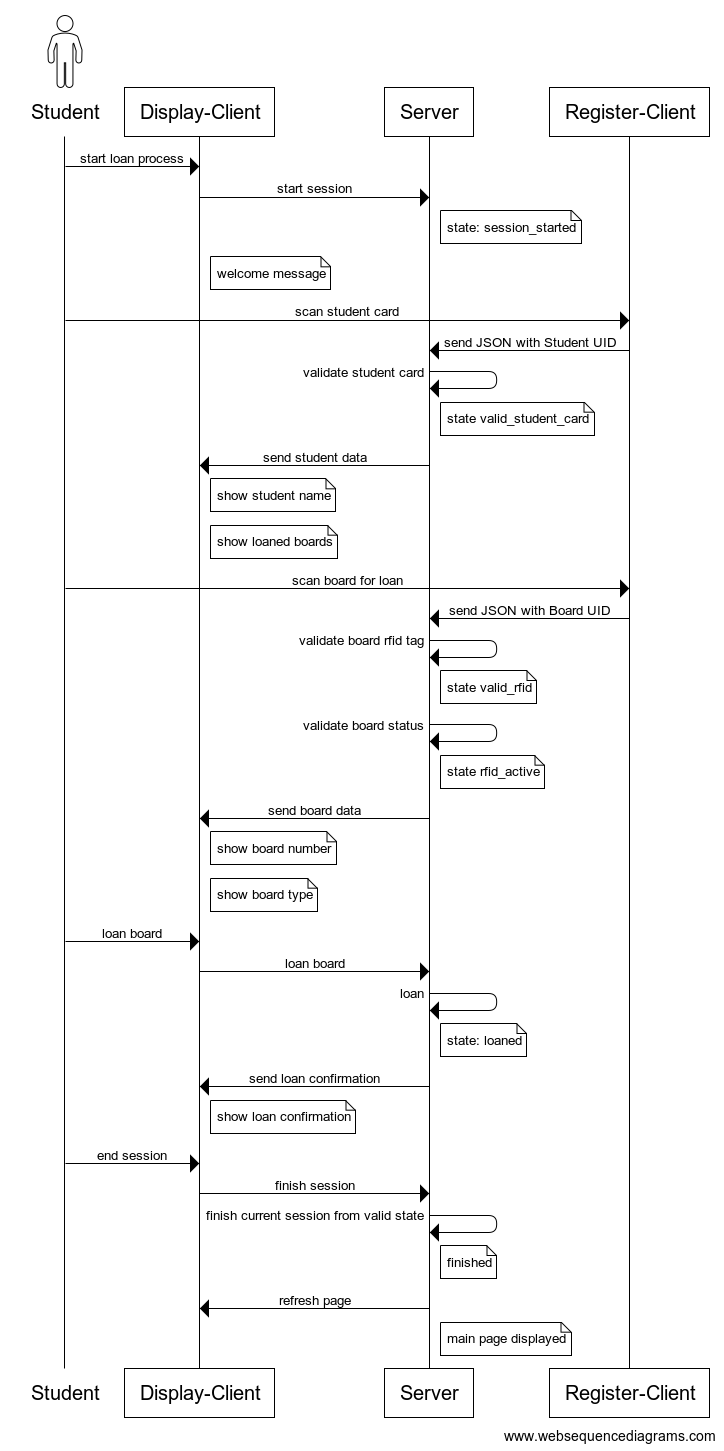
\includegraphics[width=0.8\textwidth]{gfx/seq.png}}
	\caption{Sequenzdiagramme der erfolgreichen Ausleihe der Lab-Loan Raspi Board}
	\label{fig:seq}
\end{figure}
Sequenzdiagramme beschreiben, wie und in welcher Reihenfolge die Objekte in einem System funktionieren. Diese Diagramme wird häufig verwendet, um Anforderungen an neue und vorhandene Systeme zu dokumentieren und zu verstehen. Ein Sequenzdiagramm ist so strukturiert, dass es eine Zeitleiste darstellt, die oben beginnt und nach unten abfällt, um die Sequenz der Interaktionen zu markieren. Jedes Objekt hat eine Spalte und die zwischen ihnen ausgetauschten Nachrichten werden durch Pfeile dargestellt. Diese Pfeile werden Lebensliniennotationen genannt und ein Sequenzdiagramm besteht aus mehreren dieser Lebensliniennotationen, die horizontal angeordnet sein sollten. Keine zwei Lebensliniennotationen sollten sich überlappen. Sie repräsentieren sie die verschiedenen Objekte, die während der Sequenz im System miteinander interagieren. Es ist besser kleinere Sequenzdiagramme zu zeichnen, die das Wesentliche des Anwendungsfalls erfassen
anstatt ein Sequenzdiagramm mit mehreren Objekten und Gruppen von Nachrichten zu überladen, die den Leser verwirren. In der Abschlussarbeit werden ein Sequenzdiagramm gezeigt, die auf den Abbildungen \ref{fig:seq} zu betrachten ist. Es ist ein erfolgreichen Szenario für die Ausleihe der Lab-Loan Raspi Board von einem gültigen Studierende. Das Sequenzdiagramme entspricht der oben genannte User Story \textit{"As a student, I want to loan a board so I can work at lab"}. Die meisten Kommunikation geschieht über die asynchrone Nachrichten, die verwendet werden, wenn der Nachrichtenanrufer nicht darauf wartet, dass der Empfänger die Nachricht verarbeitet und zurückkehrt, bevor er andere Nachrichten an andere Objekte im System sendet. Zum Beispiel, es wird von Register-Klient mit dem angeschlossenen RFID-Leser nicht darauf gewartet, ob die abgelesene Studentenkarte gültig ist oder ob ein Student zum Kurs zugelassen ist. Sofort die vorherigen Ablesevorgang angeschlossen wurde und JSON-Datei dem Server geschickt, steht der RFID-Leser wieder zur Verfügung und ein RFID-Tag des Boards abgelesen werden kann. Es kann sogar sein, dass anstatt erwarteten in erfolgreichen Szenario RFID-Tags eine weitere Studentenkarte abgelesen wird (z.B. nebenstehende Kumpel der Studierende aus Spaß oder wegen der Eile lässt seine Karte ablesen vor dem Beenden des laufenden Ausleihevorgang). Obwohl eine weitere Studentenkarte zu lesen aus der Sich der Zustandsmaschine nicht zugelassen ist, wird trotzdem die Karte von RFID-Reader abgelesen, eine weitere JSON-Datei zum Server geschickt und weiter RFID-Leser zum nächsten Lesen freigegeben. Est is rein die Aufgabe des Servers die ankommenden Daten zu verifizieren und den Zustandsmaschine in einem weiteren Zustand zu schalten. Die entsprechende Information mit der Begrüßung der Studierende oder Fehlermeldung wird auch vom Server generiert und dem Display-Client zum Anzeigen übergeben. Mehr über diese Vorgehensweise in entsprechenden Kapitels \ref{sec:register_client:smart}, \ref{sec:server:fsm} und \ref*{sec:display_client:js} der Implementierungsphase nachzulesen. 


\section{Systemarchitektur}
\label{sec:design:arch}
\begin{figure}
	\centering
	\fbox{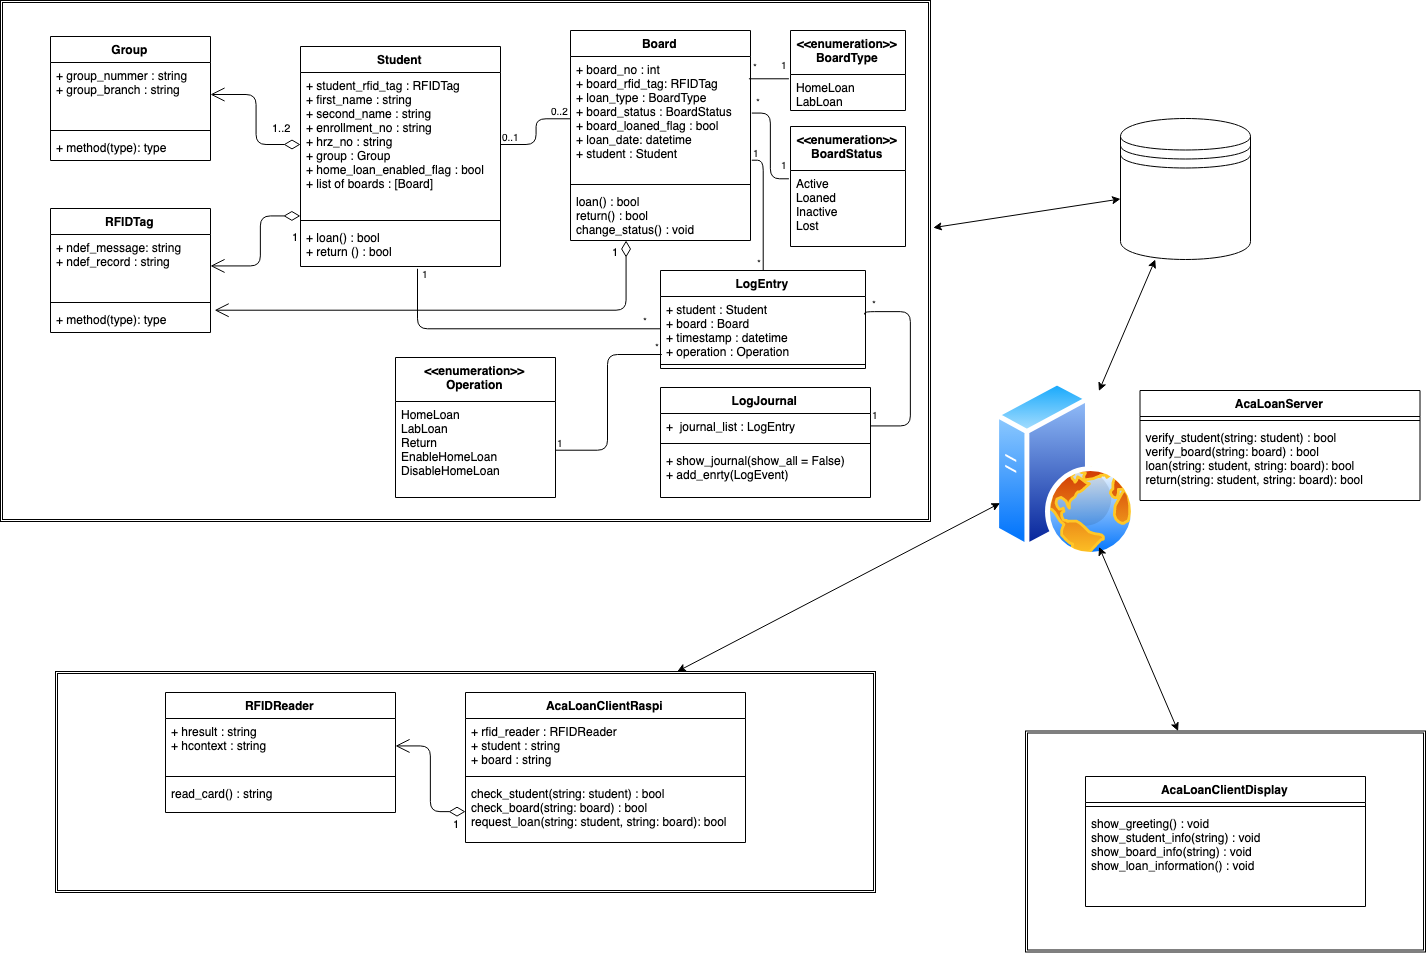
\includegraphics[width=1\textwidth]{gfx/Class_Diagram.png}}
	\caption{UML Klassendiagramm.}
	\label{fig:class}
\end{figure}
Die Architektur besteht aus den grundlegenden Beschreibungen (Ansichten),  die zeigen, aus welchen grundlegenden Teilen (Komponenten, Modulen, Layouts usw.) das System besteht und wie diese Beschreibungen zusammenhängen. Das System aus Sicht des Benutzers umfasst Artefakte in Bezug auf praktische Anwendungsphasen, Szenarien und Workflows. Das System aus Sicht des Managers oder Kunden umfasst Artefakte, die die Grenze zwischen dem System und seiner Umgebung definieren, grundlegende Funktionen und Verhaltensweisen des Systems, sowie interne und externe Benutzer. Endlich das System aus Sicht der Designer definiert physische Sicht. Dies umfasst Artefakte, die die physische Grenze des Systems, Komponenten, ihre Interaktionen zwischen interne Datenbanken und Datenstrukturen und die bei seiner Entwicklung verwendeten Standards definieren.

Während des Entwurfs, der Entwicklung und der Modernisierung eines Softwaresystems erfordert die „Reihe von Entscheidungen über seine Organisation“ (Architektur) eine ständige Diskussion mit allen Beteiligten des Projekts. Auch hier ist es wichtig, dass jeder die gleiche Vorstellung über das System von sich hat. 

Es ist offensichtlich, dass für die effektive Präsentation architektonischer Lösungen für alle interessierten Parteien eine bestimmte Methode erforderlich ist, die es ermöglicht, ihre Essenz einem möglichst breiten Personenkreis auf zugängliche, aber ausreichend detaillierte Weise zu vermitteln. Ein Klassendiagramm kann auf diese Weise dienen. Das Klassendiagramm definiert die Objekttypen im System und die verschiedenen Arten von Beziehungen, die zwischen ihnen bestehen. Es bietet eine allgemeine Ansicht einer Anwendung. Diese Modellierungsmethode kann mit fast allen objektorientierten Methoden ausgeführt werden. Das Klassendiagramm erklärt, was sind die Komponenten des Systems und wo sollen wir die Einkapselungsbarrieren platzieren. Welche Entscheidungen sind innerhalb von Komponenten zu verbergen, damit sie geändert werden können, ohne den Rest des Systems zu beeinträchtigen. Wie und was müssen die Komponenten wirklich kommunizieren. Zum Beispiel, was sollte in den Schnittstellen sein oder welches Protokoll sollte verwendet werden? Auf der Abbildung \ref{fig:class} den Zusammenhang zwischen die drei Bestandsteilen (Register-Client, Server und Display-Client) mit den Einkapselungsbarrieren zu sehen. Da es schon während der Besprechung der Aufgabestellung mit den PSE-Labor Mitbietern für eine Entwicklung mit Django Framework entschieden wurde, wird es im Klassendiagramm schon zu sehen. Die Klassen wurden am Anfang als die Django Modele geplant, die in einer SQLite Datenbank verwaltet werden. Dann muss z.B. kein Primärschlüssel in Datenbankdesign definiert werden, da es von Django eine Primärschlüssel erzeugt wird und Entwickler darüber nicht kümmern muss. Die drei Komponenten werden miteinander über HTTP-Protokoll kommunizieren. Es wird mithilfe API-Endpunkt geschehen, an dem eine Verbindung mit den drei Bestandteilen der Softwareprogramm herstellt wird. An den API-Endpunkt werden Informationsanforderungen von einer Webanwendung einem Webserver geschickt die Antwort empfangen.

\section{Endliche Zustandsmaschine}
\label{sec:design:fsm}
